\section{Основные понятия}

\subsection{Обозначения}

Ниже, мы введем обозначения, которые будут использоваться в этой работе.

\begin{itemize}
	\item $\sqcup$ обозначает дизъюнктивное объединение: используя $A\sqcup B$ вместо $A\cup B$, мы подчеркиваем, что множества $A$~и~$B$ не пересекаются. 
	\item $\oplus$ обозначает сложение по модулю~$2$.
	\item $[n]$ обозначает множество $\{1, 2, \dotsc, n\}$ (в частности, $[2^n] = \{1, 2, \dotsc, 2^n\}$).
	\item $o(\cdot), O(\cdot), \omega(\cdot), \Omega(\cdot), \Theta(\cdot)$ обозначают O~маленькое, 
	O~большое, омегу маленькую, омегу большую, и тету большую, соответственно.
	\item Для функций $f,g \colon \mathbb{Z}_{>0} \to \mathbb{R}_{>0}$, говоря, что $f(n) = 2^{O(g(n))}$, мы подразумеваем, что существует $\alpha > 0$ такая, что
	$f(n) \le 2^{\alpha \cdot g(n)}$ 
	для всех ~$n$.
	\item Для функций $f,g \colon \mathbb{Z}_{>0} \to \mathbb{R}_{>0}$, говоря, что $f(n) = 2^{o(g(n))}$,мы подразумеваем, что для любой константы $\alpha > 0$ существует натуральное число $n_0$ такое, что
	$f(n) \le 2^{\alpha \cdot g(n)}$ 
	для всех~$n > n_0$.
	\item Для функций $f,g \colon \mathbb{Z}_{>0} \to \mathbb{R}_{>0}$, говоря, что $f(n) = 2^{\Omega(g(n))}$, мы подразумеваем, что существует $\alpha > 0$ такая, что 
	$f(n) \ge 2^{\alpha \cdot g(n)}$ 
	для всех~$n$.
	\item Для функций $f,g \colon \mathbb{Z}_{>0} \to \mathbb{R}_{>0}$, говоря, что $f(n) = 2^{\omega(g(n))}$, мы подразумеваем, что для любой константы $\alpha > 0$ существует натуральное число $n_0$ такое, что 
	$f(n) \ge 2^{\alpha \cdot g(n)}$ 
	для всех~$n > n_0$.
\end{itemize}

\subsection{Вычисление Булевой Функции с Помощью КНФ}
Для булевой функции $f(x_1, \dotsc, x_n) \colon \{0,1\}^n \to \{0,1\}$, будем говорить, что КНФ~$F(x_1, \dotsc, x_n)$ \emph{вычисляет~$f$}, если $f \equiv F$, то есть, для всех $x_1, \dotsc, x_n \in \{0,1\}$, $f(x_1, \dotsc, x_n)=F(x_1, \dotsc, x_n)$.
Мы рассматриваем КНФ как набор дизъюнктов, и под \emph{размером} КНФ мы имеем ввиду число дизъюнктов.
Хорошо известно, что для любой функции~$f$ существует КНФ, вычисляющая эту функцию. Один из способов построить такую КНФ выглядит следующим образом: для каждого входа $x \in \{0,1\}^n$ такого, что $f(x)=0$, добавим в КНФ дизъюнкт длины~$n$, который не выполняется входом~$x$.

Этот метод не гарантирует, что полученная КНФ имеет минимальный размер: это было бы слишком хорошо, так как задача поиска КНФ минимального размера для булевой функции (данной в виде таблицы истинности) является NP-трудной, как доказал Масек~\cite{MasekNpComp} (смотри также \cite{DBLP:journals/siamcomp/AllenderHMPS08} и ссылки там).
Например, для функции $f(x_1,x_2)=x_1$, вышеизложенный метод производит КНФ $({x_1} \lor x_2) \land ({x_1} \lor \overline{x_2})$, в то время как сама функция $x_1$ уже в КНФ форме.

Доказано, что для многих функций, минимальная КНФ имеет экспоненциальный размер. Каноническим примером является функция четности $\PAR_n(x_1, \dotsc, x_n)=x_1 \oplus \dotsb \oplus x_n$. Важным свойством $\PAR_n$ является повышенная \emph{чувствительность}: меняя \emph{любой} бит во входе~$x \in \{0,1\}^n$, меняется значение всей функции~$\PAR_n(x)$. Именно из - за этого свойства не может быть маленькой КНФ, вычисляющей функцию $\PAR_n$.

\begin{lemma}\label{lemma:detparity}
	Минимальный размер КНФ, вычисляющей~$\PAR_n$ равен $2^{n-1}$.
\end{lemma}
\begin{proof}
	Верхняя оценка следует из метода, изложенного выше и факта, что $|\PAR_n^{-1}(0)|=2^{n-1}$.
	
	Нижняя оценка основана на факте, что любой дизъюнкт у КНФ~$F$ вычисляющей $\PAR_n$, должен содержать все переменные $x_1, \dotsc, x_n$.
	Действительно, если дизъюнкт $C \in F$ не зависит от переменной~$x_i$, то можно найти вход $x \in \{0,1\}^n$, который опровергает~$C$ (таким образом $F(x)=\PAR_n(x)=0$), и продолжит опровергать $C$ после инвертирования $x_i$. 
	Так как любой дихъюнкт~$F$ имееет ровно $n$ переменных, то он опровергает ровно один вход $x \in \{0,1\}^n$. Следовательно, $F$ должен содержать хотя бы  $|\PAR_n^{-1}(0)|=2^{n-1}$ дизъюнктов.
\end{proof}

\subsection{Кодирование Булевой Функции с Помощью КНФ}\label{sec:encodings}
Будем говорить, что КНФ~$F$ \emph{кодирует} булеву функцию $f(x_1, \dotsc, x_n)$, если следующие два условия выполняются.
\begin{enumerate}
	\item В дополнение ко входным битам $x_1, \dotsc, x_n$, $F$ также зависит от $s$~битов $y_1, \dotsc, y_s$, называемые \emph{недетерминированные входы} or \emph{дополнительные входы}.
	\item Для каждого $x \in \{0,1\}^n$, $f(x)=1$ тогда и только тогда, когда существует $y \in \{0,1\}^s$ такой, что $F(x,y)=1$. Другими словами, для всех $x \in \{0,1\}^n$,
	\begin{equation}\label{eq:enc}
		f(x) = \bigvee_{y \in \{0,1\}^s}F(x,y) \, .
	\end{equation}
\end{enumerate}
Такое представление булевой функции широко используется на практике при переводе задачи в КНФ.
Например, следующая КНФ кодирует $\PAR_4$:
\begin{multline}\label{eq:toyenc}
	(x_1 \lor x_2 \lor \overline{y_1}) \land (x_1 \lor  \overline{x_2} \lor y_1) \land (\overline{x_1} \lor x_2 \lor y_1) \land (\overline{x_1} \lor \overline{x_2} \lor \overline{y_1})
	\land
	(y_1 \lor x_3 \lor \overline{y_2}) \land\\ (y_1 \lor  \overline{x_3} \lor y_2) \land (\overline{y_1} \lor x_3 \lor y_2) \land (\overline{y_1} \lor \overline{x_3} \lor \overline{y_2})
	\land (\overline{x_4} \lor y_2) \land (x_4 \lor \overline{y_2}) \, .
\end{multline}

Этот пример обобщается следующим образом.
Чтобы закодировать $x_1 \oplus \dotsb \oplus x_n$ в виде КНФ,
надо ввести
$s \in \mathbb{Z}_{\ge 0}$~недетерминированных переменных $y_1, \dotsc, y_s$
и разделить множество входных переменных на дизъюнктивные множества размер не более $\lceil n/(s+1) \rceil$: $\{x_1, x_2, \dotsc, x_n\}=X_1 \sqcup X_2 \sqcup \dotsb \sqcup X_{s+1}$. 
Затем запишем следующие $s+1$ булевы функции в виде КНФ:
\begin{multline}\label{eq:blocks}
	\left(y_1 \equiv \bigoplus_{x \in X_1}x\right),
	\left(y_2 \equiv y_1 \oplus \bigoplus_{x \in X_2}x\right), \dotsc,\\
	\left(y_s \equiv y_{s-1} \oplus \bigoplus_{x \in X_s}x\right),
	\left(1 \equiv y_s \oplus \bigoplus_{x \in X_{s+1}}x\right).
\end{multline}
Каждая скобка может быть рассмотрена как булева функция от $k$ переменных, где $k \le \lceil n/(s+1) \rceil + 2$. Каждая такая функция имеет  $2^{k - 1}$ нулей, и поэтому может быть закодирована с помощью $2^{k - 1} \le 2^{\lceil n/(s+1) \rceil+2-1}$ дизъюнктов.
Значение для параметра~$s$ обычно определяется эксперементально. 
Например, Прествич~\cite{DBLP:journals/dam/Prestwich03} говорит, 
что лучший результат при решении задачи "minimal disagreement parity learning", используя САТ-солверы, основанные на локальном поиске, достигается при $s=10$.

Конструкция выше позволяет закодировать функцию четности в виде КНФ со следующей верхней границей на число дизъюнктов $m$.
%, число недетерминированных переменных~$s$ и ширину дизъюнктов~$k$.
\begin{description}
	\item[Ограниченный недетерминизм] используя $s \in \mathbb{Z}_{\ge 0}$~недетерминированных переменных, можно закодировать функцию четности 
%	либо
	как КНФ с не более, чем 
	\begin{equation}\label{eq:upperm}
		m \le (s+1)2^{\lceil n/(s+1) \rceil+1} \le 4(s+1)2^{n/(s+1)}
	\end{equation}
	дизъюнктами
%	, либо как~$k$-КНФ, где
%	\begin{equation}\label{eq:upperk}
%		k=2+{\lceil n/(s+1) \rceil} \le 3+n/(s+1) \, ,
%	\end{equation}
%	(следует из~\eqref{eq:blocks}).
\end{description}
	
%	\item[Unlimited nondeterminism:] one can encode parity 
%	as~a~CNF with at~most
%	\begin{equation}\label{eq:uppermtwo}
%		m \le 4n
%	\end{equation}
%	clauses
%	(to~do this, use $s=n-1$ nondeterministic variables; then, each of~$n$~functions in~\eqref{eq:blocks} can be~written in~CNF using at~most four clauses).

\subsection{Булевы Схемы и Преобразование Цейтина}\label{sec:tseitin}
Один из естественных способов получить КНФ кодировку булевой функции~$f$ следующий.
Возьмем булеву схему, вычисляющую~$f$ и применем преобразование Цейтина~\cite{zbMATH03325539}.
Мы опишем это преобразование, используя игрушечный пример.
Следующая схема вычисляет  $\PAR_{12}$ с помощью трех гейтов:
входные степени у $y_2$ и $y_3$ равны пяти, в то время как входная степень у $y_1$ равна четырем.
Схема имеем $12$ входов и $3$ гейта (один из них~---~выходной гейт), ее глубина равна трем.

\tikzstyle{gate} = [circle, draw, inner sep=0mm, minimum size=5mm]

\begin{center}
	\begin{tikzpicture}[yscale=1]
		%\draw[help lines] (1,0) grid (12,3);
		\begin{scope}[xscale=0.7, yscale=0.7]
			\foreach \n in {1,...,12}
			\node (\n) at (\n,0) {$x_{\n}$};
			\foreach \x/\y/\n/\l/\edges in {2.5/1/y1/y_1/{1,2,3,4}, 6.5/1.5/y2/y_2/{5,6,7,8,y1}, 10.5/2/y_3/y_3/{9,10,11,12,y2}} {
				\node[gate,label=above:$\l$] (\n) at (\x,\y) {$\oplus$};
				\foreach \i in \edges
				\draw[->] (\i) -- (\n);
			}
		\end{scope}
		\node[right, text width=42mm, inner sep=0mm] at (9,.75) {
			$y_1=x_1 \oplus x_2 \oplus x_3 \oplus x_4$\\
			$y_2=y_1 \oplus x_5 \oplus x_6 \oplus x_7 \oplus x_8$\\
			$y_3=y_2 \oplus x_9 \oplus x_{10} \oplus x_{11} \oplus x_{12}$
		};
	\end{tikzpicture}
\end{center}
%
Справа от схемы мы показываем функции, считающиеся каждым гейтом. 
Каждая строчка может быть переведена в КНФ.
Чтобы получить КНФ кодировку изначальной функции, надо добавить дизъюнкт $(y_3)$ к результирующей КНФ.
На самом деле, КНФ~\eqref{eq:blocks} получается ровно этим способом (после проталкивания значения выходного гейта).

\begin{observation}\label{obs:binarycircuits}
	Если функция $f \colon \{0,1\}^n \to \{0,1\}$ может быть вычислена схемой входной степени два с $g$ гейтами, тогда $f$ может быть закодирована как $3$-КНФ с $s=g$ недетерминированными переменными и $m=4g$ клозами.
\end{observation}
\begin{proof}
	Для каждого гейта~$g$ вычислим $g_1 \circ g_2$, где $\circ$~---~это бинарная булева операция, и $g_1$ вместе с $g_2$ являются прямыми предками $g$. Дальше, с помощью четырех $3$-дизъюнктов выразим факт, 
	что $g=g_1 \circ g_2$.
	(Более формально, можно рассмотреть булеву функцию $h(g, g_1, g_2)=[g=g_1 \circ g_2]$. 
	Тогда $|h^{-1}(0)|=4$, что может быть закодировано с помощью четырех $3$-дизъюнктов.)
\end{proof}

\subsection{Верхние Оценки Для Симметрических Функций}\label{upperbound}
Функции четности и голосования являются симметрическими. Напомним, что
булева функция называется симметрической, если ее значение зависит только от суммы (натуральной) входных переменных.
Чтобы закодировать любую симметрическую функцию $f(x_1, \dotsc, x_n)$ в КНФ, можно использовать кострукцию, похожую на~\eqref{eq:blocks}. 
А именно, разделим входные переменные на $t$  дизъюнктивных подмножеств размера не больше $\lceil n/t \rceil$:
$\{x_1, x_2, \dotsc, x_n\}=X_1 \sqcup X_2 \sqcup \dotsb \sqcup X_{t}$.
Пусть $Y_1, \dotsc, Y_t$ будут $t$~подмножеств, каждое из которых состоит из $\lceil \log_2 (n+1) \rceil$ недетерминированных переменных.
Под $Y_i$ будем обозначать биты натурального числа $0 \le y_i \le n$.
Затем запишем с помощью КНФ каждое из следующих тождеств:
\[
\left(y_1 \equiv \sum_{x \in X_1}x\right),
\left(y_2 \equiv y_1+\sum_{x \in X_2}x\right), 
\dotsc,
\left(y_t \equiv y_{t_1}+\sum_{x \in X_t}x\right).
\]
Тогда $y_t$ будет равен~$\sum_{i=1}^nx_i$. То есть с помощью не больше, чем  
$2^{|Y_t|}=2^{\lceil \log_2 (n+1) \rceil} \le 2n$ дополнительных дизъюнктов, мы сможем гарантировать правильное значение для~$f(x_1, \dotsc, x_n)$.
Таким образом, общее число дизъюнктов будет равно

	\[m \le t \cdot \lceil \log_2 (n+1) \rceil \cdot 2^{\lceil n/t\rceil+ \lceil \log_2 (n+1) \rceil} + 2n \, .\]
Мы получили, что для любого натурального~$t$, можно использовать $s=t \cdot \lceil \log_2 (n+1) \rceil$ недетерминированных переменных, чтобы закодировать симметрическую функцию в виде КНФ с
	\[m \le 4 \cdot s \cdot n \cdot 2^{\frac{n (\log n + 1)}{s}} + 2n\]
дизъюнктами.

Известно, что любая симметрическая функция может быть вычислена схемой (над полным бинарным базисом)
размера $4.5n+o(n)$~\cite{DBLP:journals/ipl/DemenkovKKY10}.
Наблюдение~\ref{obs:binarycircuits} дает нам, что любая симметрическая булева функция может быть закодирована в виде~$3$-КНФ 
с $4.5n+o(n)$ недетерминированными переменными и 
$18n+o(n)$ дизъюнктами.

\subsection{Схемы глубины 3}

На КНФ формулу можно смотреть как на схему глубины $2$, где выходной гейт это большой $\AND$-гейт, а все остальные гейты~---~$\OR$-гейты. Входами такой схемы как и раньше будут переменные или их отрицания. Например, следующая  схема соответствует КНФ~\eqref{eq:toyenc}. Такая схема  глубины $2$ также обозначается как  $\AND \circ \OR$ схема.


\begin{center}
	\begin{tikzpicture}[xscale=.9, yscale=.5, >=latex]
		%\draw[help lines] (0,0) grid (14,5);
		
		\foreach \n\s in {1/x_1, 2/x_2, 3/\overline{y_1},
			4/x_1, 5/\overline{x_2}, 6/y_1,
			7/\overline{x_1}, 8/x_2, 9/y_1,
			10/\overline{x_1}, 11/\overline{x_2}, 12/\overline{y_1},
			13/y_1, 14/x_3, 15/\overline{y_2},
			16/y_1, 17/\overline{x_3}, 18/y_2,
			19/\overline{y_1}, 20/x_3, 21/y_2,
			22/\overline{y_1}, 23/\overline{x_3}, 24/\overline{y_2}}
		\node (v_\n) at (0.5 * \n - 0.5, 0) {$\s$};
		
		\node (v_25) at (12.3, 0) {$y_2$};
		\node (v_26) at (12.7, 0) {$\overline{x_4}$};
		\node (v_27) at (13.7, 0) {$\overline{y_2}$};
		\node (v_28) at (14.3, 0) {$x_4$};
		
		\foreach \m in {1,...,10}
		\node[gate] (y\m) at (-1 + 1.5 * \m, 2) {$\lor$};
		
		\foreach \n in {2,...,25} {
			\def\qq{\the\numexpr\n / 3}
			\def\tt{\the\numexpr\qq}
			\def\dec{\the\numexpr\n - 1}
			\draw[->] (v_\dec) -- (y\tt);
		}
		
		\draw[->] (v_25) -- (y9);
		\draw[->] (v_26) -- (y9);
		\draw[->] (v_27) -- (y10);
		\draw[->] (v_28) -- (y10);
		
		\node[gate] (z) at (7.25, 4.5) {$\land$};
		
		\foreach \n in {1,...,10}
		\draw[->] (y\n) -- (z);
		
	\end{tikzpicture}
\end{center}

Естественным обобщением КНФ являются схемы глубины $3$:
~\emph{$\Sigma_3$-схема}~---~это просто $\OR$ некоторого количества КНФ.
В случае схемы, этим КНФ разрешенего иметь общие дизъюнкты.
\emph{$\Sigma_3$-формула}~---~это $\Sigma_3$-схема, у которой КНФ функции не имеют общих дизъюнктов
(другими словами, это схема, в которой выходная степень каждого гейта равна $1$).

Уравнение~\eqref{eq:enc} демонстрирует тесную связь между КНФ кодировками и $\OR \circ \AND \circ \OR$ схемами глубины $3$.
А именно, пусть $F(x_1, \dotsc, x_n, y_1, \dotsc, y_s)=\{C_1, \dotsc, C_m\}$ будет КНФ кодировкой булевой функции $f \colon \{0,1\}^n \to \{0,1\}$. Тогда,
$f(x)=\lor_{y \in \{0,1\}^s}F(x,y)$. 
Теперь давайте рассмотрим все возможные означивания для $y$-ов. Перебрав $2^s$ способов можно получить ~$\Sigma_3$-формулу, которая вычисляет~$f$:
\begin{equation}\label{eq:projection}
	f(x)=\bigvee_{j \in [2^s]}F_j(x) \, ,
\end{equation}
где каждая $F_j$~---~это КНФ. 
Мы будем называть это~\emph{проекцией} $F$. Например, \emph{проекция} КНФ~\eqref{eq:toyenc} выглядит следующим образом: это $\OR$ четырех КНФ.
\begin{center}
	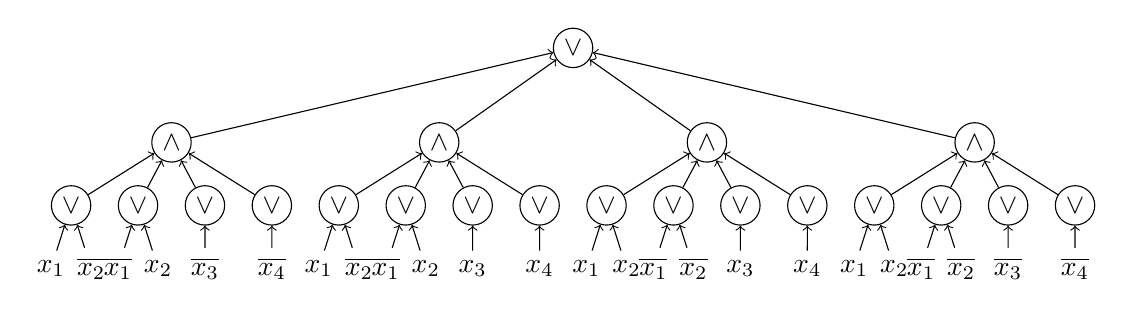
\begin{tikzpicture}[xscale=.85, yscale=.4]
		%\draw[help lines] (0,0) grid (15,7);
		
		\foreach \n\s\dx\t in {1/x_1/-0.3/0, 2/\overline{x_2}/0.3/0, 3/\overline{x_1}/-0.3/1,
			4/x_2/0.3/1, 5/\overline{x_3}/0/2, 6/\overline{x_4}/0/3,
			7/x_1/-0.3/4, 8/\overline{x_2}/0.3/4, 9/\overline{x_1}/-0.3/5,
			10/x_2/0.3/5, 11/x_3/0/6, 12/x_4/0/7,
			13/x_1/-0.3/8, 14/x_2/0.3/8, 15/\overline{x_1}/-0.3/9,
			16/\overline{x_2}/0.3/9, 17/x_3/0/10, 18/x_4/0/11,
			19/x_1/-0.3/12, 20/x_2/0.3/12, 21/\overline{x_1}/-0.3/13,
			22/\overline{x_2}/0.3/13, 23/\overline{x_3}/0/14, 24/\overline{x_4}/0/15
		}
		\node (v_\n) at (\t+\dx, 0) {$\s$};
		
		\foreach \m in {1,...,16}
		\node[circle, draw, inner sep=0mm, minimum size=5mm] (y\m) at (-1 + 1 * \m, 2) {$\lor$};
		
		\foreach \m in {1,...,4}
		\node[circle, draw, inner sep=0mm, minimum size=5mm] (z\m) at (-2.5 + 4 * \m, 4) {$\land$};
		
		\node[circle, draw, inner sep=0mm, minimum size=5mm] (q) at (7.5, 7) {$\lor$};
		
		\foreach \n in {1,...,4}
		\draw[->] (z\n) -- (q);
		
		\foreach \n\m in {1/1, 2/1, 3/1, 4/1, 5/2, 6/2, 7/2, 8/2,
			9/3, 10/3, 11/3, 12/3, 13/4, 14/4, 15/4, 16/4}
		\draw[->]  (y\n) -- (z\m);
		
		\foreach \n\m in {1/1, 2/1, 3/2, 4/2, 5/3, 6/4,
			7/5, 8/5, 9/6, 10/6, 11/7, 12/8,
			13/9, 14/9, 15/10, 16/10, 17/11, 18/12,
			19/13, 20/13, 21/14, 22/14, 23/15, 24/16}
		\draw[->] (v_\n) -- (y\m);
	\end{tikzpicture}
\end{center}
\emph{Проекция} является формулой: это OR нескольких КНФ, каждый гейт имеет выходную степень один.
Аналогично можно определить \emph{проекцию схему}: в этом случае гейтам разрешено иметь выходную степень больше, чем один; иначе говоря, КНФы могут иметь общие дизъюнкты.
Ниже приведена проекция для~\eqref{eq:toyenc}.

\begin{center}
	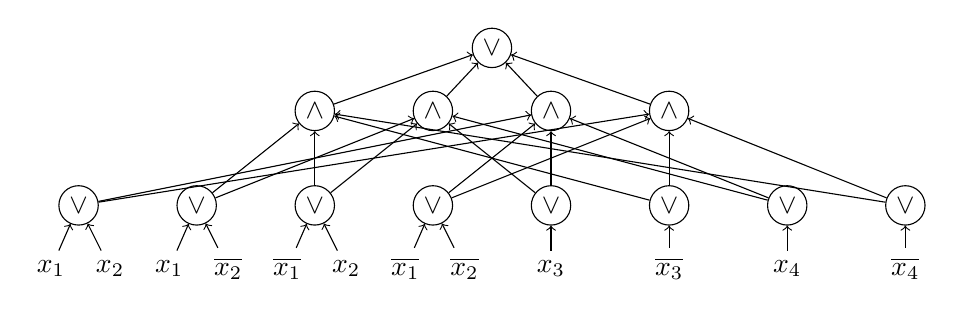
\begin{tikzpicture}[yscale=.4]
		%\draw[help lines] (0,0) grid (11,7);
		
		\foreach \n\s in {1/x_1, 2/x_2,
			3/x_1, 4/\overline{x_2},
			5/\overline{x_1}, 6/x_2,
			7/\overline{x_1}, 8/\overline{x_2}}
		\node (v_\n) at (0.75 * \n-0.6, 0) {$\s$};
		\foreach \n\s in {9/x_3, 10/\overline{x_3},
			11/x_4, 12/\overline{x_4}}
		\node (v_\n) at (1.5 * \n-7, 0) {$\s$};
		
		\foreach \m in {1,...,8}
		\node[circle, draw, inner sep=0mm, minimum size=5mm] (y\m) at (-1 + 1.5 * \m, 2) {$\lor$};
		
		\foreach \m in {1,...,4}
		\node[circle, draw, inner sep=0mm, minimum size=5mm] (z\m) at (2 + 1.5 * \m, 5) {$\land$};
		
		\node[circle, draw, inner sep=0mm, minimum size=5mm] (q) at (5.75, 7) {$\lor$};
		
		\foreach \n in {1,...,4}
		\draw[->] (z\n) -- (q);
		
		\foreach \n\m in {1/3, 1/4, 2/1, 2/2, 3/1, 3/2, 4/3, 4/4,
			5/2, 5/3, 6/1, 6/4, 7/2, 7/3, 8/1, 8/4}
		\draw[->]  (y\n) -- (z\m);
		
		\foreach \n\m in {1/1, 2/1, 3/2, 4/2, 5/3, 6/3, 7/4, 8/4,
			9/5, 10/6, 11/7, 12/8}
		\draw[->] (v_\n) -- (y\m);
		
	\end{tikzpicture}
\end{center}

Следующая лемма покажет связь между КНФ кодировками и схемами глубины $3$. 
А именно, мы покажем, что они могут быть преобразованы друг в друга.
Для удобства определим размер схемы как число гейтов, не включая выходные гейты.
В таком случае, размер КНФ формулы будет равен числу дизъюнктов (КНФ это схема глубины $2$).
$\Sigma_3(t,r)$-схема будет обозначать $\Sigma_3$-схему, 
которая имеет не больше $t$~AND гейтов на втором слое и не больше $r$~OR гейтов на третьем слое 
(то есть, размер такой схемы не больше $t+r$).

\begin{lemma}
	Пусть $F(x_1, \dotsc, x_n, y_1, \dotsc, y_s)$ будет КНФ кодировкой размера $m$
	функции
	$f \colon \{0,1\}^n \to \{0,1\}$.
	Тогда, $f$~может быть вычислена с помощью
	$\Sigma_3(2^s, m \cdot 2^s)$-формулы и с помощью $\Sigma_3(2^s,m)$-схемы.
\end{lemma}
\begin{proof}
	Пусть $F=\{C_1, \dotsc, C_m\}$. Рассмотрим проекцию $F$ равную~$\bigvee_{j \in [2^s]}F_j$,
	то есть мы перебрали все $2^s$ означиваний недетерминированных переменных
	$y_1, \dotsc, y_s$. 
	Для каждого такого означивания каждый дизъюнкт $C_i$ либо становится выполненным, 
	либо превращается в дизъюнкт $C_i' \subseteq C_i$, полученный из $C_i$ 
	удалением всех недетерминированных переменных.
	Таким образом, для каждого $j \in [2^s]$, $F_j \subseteq \{C_1', \dotsc, C_m'\}$.
	Соответствующая $\Sigma_3$-формула содержит не более $2^s+m2^s$ гейтов:
	есть $2^s$ гейтов для каждой $F_j$, каждая $F_j$содержит не больше $m$ дизъюнктов.
	Соответствующая $\Sigma_3$-схема содержит не более, чем $2^s+m$ гейтов:
	есть $2^s$ гейтов для каждой $F_j$, и $m$~гейтов для $C_1', \dotsc, C_m'$
	(каждая $F_j$ выбирает какие из этих $m$~дизъюнктов содержать).
\end{proof}

Ниже мы покажем обратное преобразование.

\begin{lemma}\label{lemma:circuit2encoding}
	\begin{enumerate}
		\item Пусть $C$~будет~$\Sigma_3(t,r)$-формулой, вычисляющей булеву функцию $f \colon \{0,1\}^n \to \{0,1\}$. 
		Тогда,
		$f$~может быть закодирована как КНФ с $\lceil \log t \rceil$ недетерминированными переменными размера $r$.
		\item Пусть $C$~будет $\Sigma_3(t,r)$-схема, вычисляющая булеву функцию $f \colon \{0,1\}^n \to \{0,1\}$. Тогда,
		$f$~может быть закодирована как КНФ с $\lceil \log t \rceil$ недетерминированными переменными размера~$rt$.
	\end{enumerate}
\end{lemma}

\begin{proof}
	\begin{enumerate}
		\item Пусть $C=F_1 \lor \dotsb \lor F_{t}$ будет $\Sigma_3$-формулой (то есть, $r=\size(F_1)+\dotsb+\size(F_{t})$). Введем $s=\lceil\log t\rceil$ недетерминированных переменных $y_1, \dotsc, y_s$. 
		Теперь для каждого означивания $y_1, \dotsc, y_s$ возьмем соответствующую КНФ $F_i$ ($1 \le i \le 2^s$ это уникальное целое число, соответствующее означиванию) и добавим
		$y_i$с правильным знаком в каждый дизъюнкт функции $F_i$.
		Назовем получившуюся КНФ $F_i'$. Тогда, $F=F_1'\land \dotsb \land F_{2^s}'$ кодирует $f$, и $F$~имеет не больше $r$~дизъюнктов.

		\item Преобразуем $\Sigma_3(t,r)$-схему $C$ в $\Sigma_3(t,rt)$-формулу $C'$ следующим образом:
		создадим раздельные копии каждого гейта соответствующего дизъюнкту в каждой из $2^s$ CNFs. Используя пункт $1$, мы получим требуемую верхнюю оценку $rt$.

	\end{enumerate}
	
	
	
\end{proof}
